\chapter{振动引论}
\intro{本章介绍振动的基本概念，包括振动的定义与分类、振动系统离散化的思想、简谐振动的基本理论、振动系统的三类基本元件（质量、弹簧、阻尼），以及能量法和D'Alembert原理。这些内容是后续各章分析具体振动问题的基础。}

%=====================================================================
\section{振动的定义与分类}
%=====================================================================

\subsection{振动的定义}

\textbf{振动}（Vibration）是指物体在其平衡位置附近所做的往复运动。更广义地说，振动是系统的一个状态变量围绕某一参考值（通常是平衡位置）随时间做交替变化的过程。振动的本质是系统中存在恢复力和惯性（或电感和电容等类比元件），使得能量在两种形式之间周期性地转换。

从数学角度看，振动表现为系统响应 $x(t)$ 是关于时间 $t$ 的周期函数或准周期函数。振动的三要素为：
\begin{itemize}
    \item \textbf{振幅}：振动物体偏离平衡位置的最大距离
    \item \textbf{频率}：单位时间内完成全振动的次数
    \item \textbf{相位}：描述振动状态的参数
\end{itemize}

\subsection{振动的分类}

\subsubsection{按激励方式分类}

\begin{enumerate}
    \item \textbf{自由振动}（Free Vibration）：系统在初始激励（初始位移或初始速度）后，不再受外界持续激励，仅靠系统自身的恢复力和惯性维持的振动。例如：敲击音叉后的振动。
    \begin{myformula}
        \[
        m\ddot{x} + kx = 0
        \]
    \end{myformula}
    
    \item \textbf{强迫振动}（Forced Vibration）：系统在持续外部激励（如周期力、基础振动）作用下产生的振动。例如：发动机运转时引起的车身振动。
    \begin{myformula}
        \[
        m\ddot{x} + kx = F_0\sin\omega t
        \]
    \end{myformula}
    
    \item \textbf{自激振动}（Self-Excited Vibration）：系统利用自身运动从非振荡能量源中获取能量来维持的振动。例如：小提琴弦的振动、机翼颤振。
    
    \item \textbf{参数振动}（Parametric Vibration）：系统的某个参数（如刚度或质量）随时间周期性变化引起的振动。例如：荡秋千时人体重心的升降改变了等效摆长。
\end{enumerate}

\subsubsection{按阻尼情况分类}

\begin{enumerate}
    \item \textbf{无阻尼振动}（Undamped Vibration）：理想情况下忽略一切能量耗散的振动模型。系统的机械能守恒，振幅不随时间衰减。
    \begin{myformula}
        \[
        m\ddot{x} + kx = 0
        \]
    \end{myformula}
    
    \item \textbf{有阻尼振动}（Damped Vibration）：考虑系统中能量耗散的振动。振幅随时间逐渐减小，直至振动消失。
    \begin{myformula}
        \[
        m\ddot{x} + c\dot{x} + kx = 0
        \]
    \end{myformula}
    
    根据阻尼的大小，又可分为：
    \begin{itemize}
        \item 欠阻尼（Underdamped）：$\zeta < 1$，系统做衰减的往复振动
        \item 临界阻尼（Critically Damped）：$\zeta = 1$，系统以最快的速度回到平衡位置而无振荡
        \item 过阻尼（Overdamped）：$\zeta > 1$，系统缓慢地返回平衡位置而无振荡
    \end{itemize}
\end{enumerate}

\subsubsection{按系统特性分类}

\begin{enumerate}
    \item \textbf{线性振动}（Linear Vibration）：系统的恢复力与位移成正比，阻尼力与速度成正比，系统的运动方程是线性常微分方程。满足叠加原理。
    \begin{myformula}
        \[
        m\ddot{x} + c\dot{x} + kx = F(t)
        \]
    \end{myformula}
    
    \item \textbf{非线性振动}（Nonlinear Vibration）：系统中存在非线性恢复力（如大变形弹簧、几何非线性）或非线性阻尼，运动方程为非线性微分方程。不满足叠加原理。常见的非线性振动包括：
    \begin{itemize}
        \item Duffing 方程：$\ddot{x} + \delta\dot{x} + \alpha x + \beta x^3 = F\cos\omega t$
        \item van der Pol 方程：$\ddot{x} - \varepsilon(1-x^2)\dot{x} + x = 0$
    \end{itemize}
\end{enumerate}

\subsubsection{按激励特性分类}

\begin{enumerate}
    \item \textbf{确定性振动}（Deterministic Vibration）：激励是时间的确定函数，系统响应可以精确预测。
    \begin{itemize}
        \item 简谐激励：$F(t) = F_0\sin\omega t$
        \item 周期激励：$F(t) = F(t+T)$
        \item 非周期激励：冲击载荷、阶跃载荷
    \end{itemize}
    
    \item \textbf{随机振动}（Random Vibration）：激励是随机的，不能用确定的时间函数描述，只能用统计方法（功率谱密度、均方值等）分析系统响应。例如：路面不平度引起的汽车振动、地震引起的建筑振动。
\end{enumerate}

%=====================================================================
\section{振动系统的离散化}
%=====================================================================

\subsection{连续系统与离散系统}

实际的工程结构（如梁、板、壳）都是具有连续分布的质量和弹性的连续系统（Continuous System）。连续系统的振动问题理论上需要无穷多个广义坐标来描述，其运动方程为偏微分方程。例如，均匀梁的横向自由振动方程为：
\begin{myformula}
    \[
    EI\frac{\partial^4 y}{\partial x^4} + \rho A\frac{\partial^2 y}{\partial t^2} = 0
    \]
\end{myformula}

然而，连续系统的精确解往往难以获得，且计算复杂。工程中常采用\textbf{离散化}的方法，将连续系统转化为有限自由度的离散系统（Discrete System）来分析。

\subsection{离散化的基本思路}

离散化的核心思想是将连续分布的参数（质量、刚度、阻尼）\textbf{集中}到有限个点上，用有限个广义坐标描述系统的运动。主要方法有：

\begin{enumerate}
    \item \textbf{集中质量法}（Lumped Mass Method）：将分布质量集中到若干离散点上，各点之间用无质量的弹性元件连接。质量矩阵为对角阵。
    
    \item \textbf{广义坐标法}（Generalized Coordinate Method / 假设模态法）：将连续系统的位移表示为一组基函数（试函数）的线性组合：
    \begin{myformula}
        \[
        y(x,t) = \sum_{i=1}^{n} q_i(t)\phi_i(x)
        \]
    \end{myformula}
    其中 $\phi_i(x)$ 为满足边界条件的试函数（如振型函数），$q_i(t)$ 为广义坐标。通过 Lagrange 方程或 Galerkin 方法得到关于 $q_i(t)$ 的常微分方程组。
    
    \item \textbf{有限单元法}（Finite Element Method, FEM）：将连续体划分为有限个单元，在单元内假设位移模式（形函数），通过能量原理建立单元的运动方程，再组装为整体方程。这是现代工程分析中最通用的离散化方法。
\end{enumerate}

\subsection{自由度}

\textbf{自由度}（Degree of Freedom, DOF）是指完全确定系统位置所需的独立坐标数。例如：
\begin{itemize}
    \item 弹簧-质量系统：1 个自由度
    \item 平面双摆：2 个自由度
    \item 空间刚体：6 个自由度（3 个平动 + 3 个转动）
\end{itemize}

离散后系统的自由度数为 $n$ 时，其运动方程为一组 $n$ 个二阶常微分方程。

%=====================================================================
\section{简谐振动基础}
%=====================================================================

\subsection{简谐运动的定义}

\textbf{简谐运动}（Simple Harmonic Motion, SHM）是最基本、最重要的周期性运动形式。它是物体在恢复力与位移成正比的条件下所做的运动。其数学表达式为：
\begin{myformula}
    \[
    x(t) = A\sin(\omega t + \phi)
    \]
\end{myformula}
或等价地：
\begin{myformula}
    \[
    x(t) = A\cos(\omega t + \phi')
    \]
\end{myformula}

其中：
\begin{itemize}
    \item $A$ —— \textbf{振幅}（Amplitude），物体偏离平衡位置的最大距离，恒为正
    \item $\omega$ —— \textbf{角频率}（Angular Frequency），单位：$\text{rad/s}$
    \item $\phi$ —— \textbf{初相位}（Initial Phase），$t=0$ 时刻的相位角
\end{itemize}

简谐运动的速度和加速度分别为：
\begin{myformula}
    \[
    \dot{x}(t) = \omega A\cos(\omega t + \phi) = \omega A\sin(\omega t + \phi + \frac{\pi}{2})
    \]
\end{myformula}
\begin{myformula}
    \[
    \ddot{x}(t) = -\omega^2 A\sin(\omega t + \phi) = -\omega^2 x(t)
    \]
\end{myformula}

由加速度表达式可得简谐运动的特征方程：
\begin{myformula}
    \[
    \ddot{x} + \omega^2 x = 0
    \]
\end{myformula}

\subsection{简谐运动的基本参数关系}

\begin{itemize}
    \item \textbf{周期} $T$：完成一次全振动所需的时间
    \begin{myformula}
        \[
        T = \frac{2\pi}{\omega}
        \]
    \end{myformula}
    
    \item \textbf{频率} $f$：单位时间内完成全振动的次数（单位：$\text{Hz} = \text{s}^{-1}$）
    \begin{myformula}
        \[
        f = \frac{1}{T} = \frac{\omega}{2\pi}
        \]
    \end{myformula}
    
    \item \textbf{角频率} $\omega$：$2\pi$ 秒内完成全振动的次数（单位：$\text{rad/s}$）
    \begin{myformula}
        \[
        \omega = 2\pi f = \frac{2\pi}{T}
        \]
    \end{myformula}
\end{itemize}

\textbf{例 1.1}：已知某简谐振动周期 $T = 0.2\,\text{s}$，振幅 $A = 0.05\,\text{m}$，初相位 $\phi = \pi/6$。求角频率、频率和 $t=0.1\,\text{s}$ 时的位移。

\textbf{解}：
\[
\omega = \frac{2\pi}{T} = \frac{2\pi}{0.2} = 10\pi \approx 31.42\,\text{rad/s},\quad 
f = \frac{1}{T} = 5\,\text{Hz}
\]
\[
x(0.1) = 0.05\sin(10\pi \times 0.1 + \pi/6) = 0.05\sin(\pi + \pi/6) = 0.05\sin(7\pi/6) = -0.025\,\text{m}
\]

\subsection{旋转矢量法（相量法）}

旋转矢量法是简谐运动的一种几何表示方法。设想一个长度为 $A$ 的矢量 $\vec{OP}$ 以匀角速度 $\omega$ 绕原点 $O$ 逆时针旋转，则矢量端点 $P$ 在 $x$ 轴上的投影即为简谐运动 $x = A\sin(\omega t + \phi)$。

\begin{center}
\begin{tikzpicture}[scale=1.3]
    % 坐标轴
    \draw[-Stealth] (-2.5,0) -- (2.5,0) node[right] {$x$};
    \draw[-Stealth] (0,-2.5) -- (0,2.5) node[above] {$y$};
    
    % 参考圆
    \draw[dashed, gray] (0,0) circle (2);
    
    % 旋转矢量
    \draw[-Stealth, very thick, blue] (0,0) -- (1.732,1) node[midway, above] {$A$};
    
    % 投影线
    \draw[dashed, red] (1.732,1) -- (1.732,0);
    \draw[dashed, red] (0,1) -- (1.732,1);
    
    % 角度标注
    \draw[-Stealth] (0.5,0) arc (0:30:0.5) node[midway, right] {$\omega t+\phi$};
    
    % 投影点
    \fill[red] (1.732,0) circle (0.05) node[below] {$x(t)$};
    
    % 端点
    \fill[blue] (1.732,1) circle (0.05) node[above right] {$P$};
    
    % 原点
    \fill (0,0) circle (0.05) node[below left] {$O$};
    
    % 位移波形示意
    \draw[-Stealth, red, thick] (1.732,0) -- (1.732,0.3);
\end{tikzpicture}
\end{center}

旋转矢量法的优点：
\begin{itemize}
    \item 直观显示振幅 $A$、角频率 $\omega$、相位 $\omega t + \phi$
    \item 便于进行简谐量的合成与分解（矢量相加）
    \item 初相位 $\phi$ 即为 $t=0$ 时旋转矢量与 $x$ 轴（或参考轴）的夹角
\end{itemize}

\subsection{简谐运动的复数表示法}

利用 Euler 公式 $e^{i\theta} = \cos\theta + i\sin\theta$，简谐运动可以用复数形式表示：
\begin{myformula}
    \[
    x(t) = \Re\{A e^{i(\omega t + \phi)}\} = \Re\{\bar{A} e^{i\omega t}\}
    \]
\end{myformula}
其中 $\bar{A} = A e^{i\phi}$ 称为\textbf{复振幅}（Complex Amplitude），它同时包含了振幅和相位信息。

复数表示的优势：
\begin{itemize}
    \item 将三角函数的运算转化为复数的代数运算
    \item 微分和积分操作简便：$\frac{d}{dt}e^{i\omega t} = i\omega e^{i\omega t}$
    \item 在频域分析中广泛使用，如频率响应函数
\end{itemize}

在复数表示中，速度和加速度为：
\begin{myformula}
    \[
    \dot{x}(t) = \Re\{i\omega \bar{A} e^{i\omega t}\},\quad
    \ddot{x}(t) = \Re\{-\omega^2 \bar{A} e^{i\omega t}\}
    \]
\end{myformula}

注意：物理量始终是复数的实部（或虚部）。在稳态分析中，约定使用实部 $\Re\{\cdot\}$;线性运算中可先对复数进行运算，最后取实部。

%=====================================================================
\section{振动系统的元件}
%=====================================================================

振动系统由三种基本元件构成：质量（惯量）元件、弹簧（刚度）元件和阻尼（耗散）元件。任何复杂的振动系统都可以等价地由这三种基本元件的组合来表示。

\subsection{质量/惯量元件}

质量元件是储存\textbf{动能}的元件。它反映系统的惯性特性。

\begin{itemize}
    \item \textbf{平动}：根据 Newton 第二定律
    \begin{myformula}
        \[
        F = m\ddot{x} = m a
        \]
    \end{myformula}
    其中 $m$ 为质量（$\text{kg}$），$\ddot{x}$ 为加速度（$\text{m/s}^2$），$F$ 为作用力（$\text{N}$）。
    
    \item \textbf{转动}：根据 Euler 方程
    \begin{myformula}
        \[
        T = J\ddot{\theta} = J\alpha
        \]
    \end{myformula}
    其中 $J$ 为转动惯量（$\text{kg}\cdot\text{m}^2$），$\ddot{\theta}$ 为角加速度（$\text{rad/s}^2$），$T$ 为转矩（$\text{N}\cdot\text{m}$）。
\end{itemize}

质量元件是\textbf{绝对}元件——其运动需参照惯性参考系（大地）。

\subsection{弹簧元件}

弹簧元件是储存\textbf{势能}的元件。它反映系统的弹性恢复能力。

\subsubsection{线性弹簧}

在线性范围内，弹簧力与变形成正比（Hooke 定律）：
\begin{myformula}
    \[
    F = kx = k(x_2 - x_1)
    \]
\end{myformula}
其中 $k$ 为弹簧刚度（$\text{N/m}$），$x$ 为相对变形量。

弹簧元件是\textbf{相对}元件——其力依赖于两端点的相对位移。

弹簧中存储的势能为：
\begin{myformula}
    \[
    V = \frac{1}{2}kx^2
    \]
\end{myformula}

\subsubsection{等效弹簧}

当多个弹簧组合使用时，可以简化为一个等效弹簧 $k_{eq}$。

\textbf{串联弹簧}：各弹簧受力相同，总变形为各弹簧变形之和。
\begin{myformula}
    \[
    \frac{1}{k_{eq}} = \frac{1}{k_1} + \frac{1}{k_2} + \cdots + \frac{1}{k_n} = \sum_{i=1}^{n}\frac{1}{k_i}
    \]
\end{myformula}

\begin{center}
\begin{tikzpicture}[scale=1.0]
    % 串联弹簧示意图
    \fill[vibWall] (0-0.2,0-0.8) rectangle (0+0.2,0+0.8);
    
    \draw[thick] (0.3,0.5) -- (0.3,-0.5);
    \draw[decorate,decoration={coil,aspect=0.6,amplitude=4,segment length=8}] (0.3,0) -- (1.8,0) node[midway,above] {$k_1$};
    \fill[draw,circle,inner sep=2pt] (1.8,0) circle (0.1);
    \draw[decorate,decoration={coil,aspect=0.6,amplitude=4,segment length=8}] (1.8,0) -- (3.3,0) node[midway,above] {$k_2$};
    \fill[draw,circle,inner sep=2pt] (3.3,0) circle (0.1);
    \draw[decorate,decoration={coil,aspect=0.6,amplitude=4,segment length=8}] (3.3,0) -- (4.8,0) node[midway,above] {$k_3$};
    
    \draw (5.0,0) node[right] {$\Rightarrow$};
    \fill[vibWall] (5.3-0.2,0-0.8) rectangle (5.3+0.2,0+0.8);
    \draw[decorate,decoration={coil,aspect=0.6,amplitude=4,segment length=8}] (5.6,0) -- (7.5,0) node[midway,above] {$k_{eq}$};
    
    \node at (2.4,-1.2) {$\displaystyle\frac{1}{k_{eq}} = \sum\frac{1}{k_i}$};
\end{tikzpicture}
\end{center}

\textbf{并联弹簧}：各弹簧变形相同，总力为各弹簧力之和。
\begin{myformula}
    \[
    k_{eq} = k_1 + k_2 + \cdots + k_n = \sum_{i=1}^{n}k_i
    \]
\end{myformula}

\begin{center}
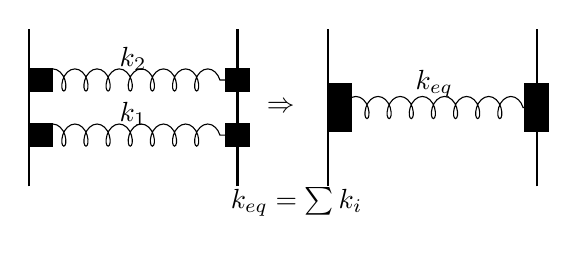
\begin{tikzpicture}[scale=1.0]
    % 并联弹簧示意图
    \draw[thick] (0,-1) -- (0,1);
    \draw[fill] (0,-0.5) rectangle (0.3,-0.2);
    \draw[fill] (0,0.5) rectangle (0.3,0.2);
    
    \draw[decorate,decoration={coil,aspect=0.6,amplitude=4,segment length=8}] (0.15,-0.35) -- (2.5,-0.35) node[midway,above] {$k_1$};
    \draw[decorate,decoration={coil,aspect=0.6,amplitude=4,segment length=8}] (0.15,0.35) -- (2.5,0.35) node[midway,above] {$k_2$};
    
    \draw[fill] (2.5,-0.5) rectangle (2.8,-0.2);
    \draw[fill] (2.5,0.5) rectangle (2.8,0.2);
    \draw[thick] (2.65,-1) -- (2.65,1);
    
    \draw (3.2,0) node {$\Rightarrow$};
    
    \draw[thick] (3.8,-1) -- (3.8,1);
    \draw[fill] (3.8,-0.3) rectangle (4.1,0.3);
    \draw[decorate,decoration={coil,aspect=0.6,amplitude=4,segment length=8}] (4.0,0) -- (6.3,0) node[midway,above] {$k_{eq}$};
    \draw[fill] (6.3,-0.3) rectangle (6.6,0.3);
    \draw[thick] (6.45,-1) -- (6.45,1);
    
    \node at (3.4,-1.2) {$k_{eq} = \sum k_i$};
\end{tikzpicture}
\end{center}

\subsection{阻尼元件}

阻尼元件是\textbf{耗散能量}的元件。它将机械能转化为热能或其他形式的能量。阻尼力总是与运动方向相反。

\subsubsection{粘性阻尼}

粘性阻尼（Viscous Damping）是最常用的阻尼模型，阻尼力与速度成正比：
\begin{myformula}
    \[
    F_d = c\dot{x}
    \]
\end{myformula}
其中 $c$ 为阻尼系数（$\text{N}\cdot\text{s/m}$），方向与速度相反。

粘性阻尼一个周期内的耗散能量为：
\begin{myformula}
    \[
    \Delta W_d = \oint c\dot{x}\,dx = \int_0^T c\dot{x}^2\,dt
    \]
\end{myformula}

\subsubsection{库仑阻尼}

库仑阻尼（Coulomb Damping）即干摩擦阻尼，阻尼力的大小恒定，方向与速度相反：
\begin{myformula}
    \[
    F_d = \mu N \cdot \sgn(\dot{x})
    \]
\end{myformula}
其中 $\mu$ 为摩擦系数，$N$ 为正压力，$\sgn(\dot{x})$ 为符号函数。

\subsubsection{结构阻尼}

结构阻尼（Structural Damping / Hysteretic Damping）是材料内部分子摩擦引起的能量耗散，其阻尼力与位移成正比，但与速度同相：
\begin{myformula}
    \[
    F_d = \frac{h}{\omega}\dot{x}
    \]
\end{myformula}
或等价地表示为复刚度：$k^* = k(1 + i\eta)$，其中 $\eta$ 为损耗因子。

\subsubsection{阻尼力-速度关系对比}

\begin{center}
\begin{tikzpicture}[scale=1.5]
    % 坐标轴
    \draw[-Stealth] (-3.0,0) -- (3.0,0) node[right] {$\dot{x}$};
    \draw[-Stealth] (0,-2.0) -- (0,2.0) node[above] {$F_d$};
    
    % 粘性阻尼：直线
    \draw[blue, very thick, domain=-2.5:2.5, samples=50] plot (\x, {0.6*\x});
    \node[blue] at (2.0,1.6) {粘性阻尼};
    
    % 库仑阻尼：阶跃
    \draw[red, very thick] (-2.5,-0.8) -- (0,-0.8);
    \draw[red, very thick] (0,0.8) -- (2.5,0.8);
    \fill[red, draw=red] (0,0.8) circle (0.05);
    \fill[red, draw=red, fill=white] (0,-0.8) circle (0.05);
    \node[red] at (-2.0,0.5) {库仑阻尼};
    
    % 结构阻尼：椭圆
    \draw[green!60!black, very thick, domain=-2.5:2.5, samples=50] plot (\x, {0.3*\x + 0.5*sin(100*\x)});
    \node[green!60!black] at (1.0,-1.0) {结构阻尼};
    
    \node[below left] at (0,0) {$O$};
\end{tikzpicture}
\end{center}

%=====================================================================
\section{能量法}
%=====================================================================

\subsection{动能与势能}

对于单自由度系统，系统的机械能由动能 $T$ 和势能 $V$ 组成。

\textbf{动能}：
\begin{myformula}
    \[
    T = \frac{1}{2}m\dot{x}^2 \quad (\text{平动}),\qquad
    T = \frac{1}{2}J\dot{\theta}^2 \quad (\text{转动})
    \]
\end{myformula}

\textbf{势能}：
\begin{myformula}
    \[
    V = \frac{1}{2}kx^2 \quad (\text{弹性势能}),\qquad
    V = mgh \quad (\text{重力势能})
    \]
\end{myformula}

对于无阻尼自由振动系统，满足\textbf{机械能守恒}：
\begin{myformula}
    \[
    T + V = \text{const}
    \]
\end{myformula}

\subsection{耗散能}

有阻尼时，阻尼力对系统做负功，导致机械能减少。一个振动周期内的\textbf{耗散能}为：
\begin{myformula}
    \[
    \Delta W_d = \oint F_d\,dx
    \]
\end{myformula}

对于粘性阻尼 $F_d = c\dot{x}$ 和简谐运动 $x = X\sin\omega t$：
\begin{myformula}
    \[
    \Delta W_d = \int_0^{2\pi/\omega} c\dot{x}^2\,dt
                = cX^2\omega^2\int_0^{2\pi/\omega}\cos^2\omega t\,dt
                = \pi c\omega X^2
    \]
\end{myformula}

\subsection{Rayleigh 能量法}

Rayleigh 能量法是求系统固有频率的近似方法。其基本思想是：\textbf{保守系统中最大动能等于最大势能}。

对单自由度系统，假设运动形式为 $x(t) = X\sin\omega_n t$，则：
\begin{myformula}
    \[
    T_{\max} = \frac{1}{2}m(\omega_n X)^2,\qquad V_{\max} = \frac{1}{2}kX^2
    \]
    \[
    T_{\max} = V_{\max} \quad\Rightarrow\quad \frac{1}{2}m\omega_n^2 X^2 = \frac{1}{2}kX^2
    \]
    \[
    \omega_n = \sqrt{\frac{k}{m}}
    \]
\end{myformula}

对于连续系统或复杂离散系统，先假设一个合理的振型函数 $y(x,t) = \phi(x)\sin\omega t$，计算系统的最大动能和最大势能，由 $T_{\max} = V_{\max}$ 得到固有频率的近似值。

\textbf{例 1.2}（Rayleigh 法求悬臂梁固有频率）：设悬臂梁长度 $L$，弯曲刚度 $EI$，单位长度质量 $\rho A$。假设静变形曲线为振型：
\[
\phi(x) = \frac{x^2}{L^2}\left(3 - \frac{x}{L}\right) \quad (\text{尖端集中力下的挠曲线})
\]
则可计算得到：
\[
\omega_n^2 = \frac{\displaystyle\int_0^L EI[\phi''(x)]^2\,dx}{\displaystyle\int_0^L \rho A[\phi(x)]^2\,dx}
\]

Rayleigh 法的精度取决于假设振型与真实振型的接近程度。通常使用静变形曲线作为假设振型可得到较好的近似结果。

\subsection{Rayleigh-Ritz 法}

Rayleigh 法的推广——Ritz 法：将假设振型写成多个基函数的线性组合：
\[
\phi(x) = \sum_{i=1}^{n} a_i\psi_i(x)
\]
其中 $\psi_i(x)$ 为满足几何边界条件的试函数，$a_i$ 为待定系数。将系统的最大动能和最大势能表示为 $a_i$ 的函数，由 $\partial(T_{\max} - V_{\max})/\partial a_i = 0$ 得到一组关于 $a_i$ 的齐次代数方程，由系数行列式为零即可求出各阶固有频率的近似值。

%=====================================================================
\section{D'Alembert 原理}
%=====================================================================

\subsection{原理表述}

D'Alembert 原理（D'Alembert's Principle）是将动力学问题转化为静力学问题的一种方法。其核心思想是：

\textbf{在运动的任何瞬间，当在质点系上施加假想的惯性力 $(-m\ddot{x})$ 后，该质点系可以视为处于平衡状态。}

数学表述为：
\begin{myformula}
    \[
    \sum(F_i - m_i\ddot{r}_i)\cdot\delta r_i = 0
    \]
\end{myformula}
其中 $F_i$ 为作用于第 $i$ 个质点上的主动力和约束反力，$-m_i\ddot{r}_i$ 为惯性力，$\delta r_i$ 为虚位移。

\subsection{在振动分析中的应用}

对于单自由度弹簧-质量系统，应用 D'Alembert 原理：

\begin{enumerate}
    \item 考虑作用于质量 $m$ 上的全部力：弹性恢复力 $-kx$、阻尼力 $-c\dot{x}$、外力 $F(t)$
    \item 引入惯性力 $-m\ddot{x}$
    \item 由 D'Alembert 原理，"平衡"条件为：
    \begin{myformula}
        \[
        F(t) - kx - c\dot{x} - m\ddot{x} = 0
        \]
    \end{myformula}
\end{enumerate}

整理得运动方程：
\begin{myformula}
    \[
    m\ddot{x} + c\dot{x} + kx = F(t)
    \]
\end{myformula}

\subsection{与 Newton 法的比较}

\begin{itemize}
    \item Newton 法：从加速度出发，建立力与加速度的关系（动力学方程）
    \item D'Alembert 法：将动力学问题转化为"平衡"问题，形式上与静力学一致，便于使用虚功原理和能量法
    \item 在复杂多体系统中，D'Alembert 原理配合虚位移原理，可以方便地导出 Lagrange 方程
\end{itemize}

\subsection{广义 D'Alembert 原理与 Lagrange 方程}

由 D'Alembert 原理和虚功原理可以推导出分析力学中的\textbf{Lagrange 方程}：
\begin{myformula}
    \[
    \frac{d}{dt}\left(\frac{\partial T}{\partial \dot{q}_i}\right) - \frac{\partial T}{\partial q_i} + \frac{\partial V}{\partial q_i} = Q_i^{\text{nc}}
    \]
\end{myformula}
其中 $q_i$ 为广义坐标，$T$ 为动能，$V$ 为势能，$Q_i^{\text{nc}}$ 为非保守广义力。Lagrange 方程是建立复杂振动系统运动方程的有力工具。

%=====================================================================
\section{振动分析的总体框架}
%=====================================================================

振动分析通常遵循以下步骤：
\begin{enumerate}
    \item \textbf{物理建模}：将实际工程问题抽象为物理模型，确定系统的质量、刚度、阻尼参数
    \item \textbf{数学建模}：建立运动微分方程（Newton 法、D'Alembert 法、Lagrange 方程、能量法等）
    \item \textbf{求解分析}：求解运动方程，分析系统的自由振动特性（固有频率、振型）和强迫振动响应
    \item \textbf{参数研究}：分析各参数对系统响应的影响，进行参数敏感性分析和优化
    \item \textbf{实验验证}：通过实验测试验证理论分析的正确性
\end{enumerate}

\subsection{小结}

本章介绍了振动的基本概念和分类方法，阐明了简谐振动的数学描述及其几何和复数表示。通过对三类基本振动元件（质量、弹簧、阻尼）的物理特性及其数学模型的讨论，以及对能量法和 D'Alembert 原理的介绍，为后续章节中具体振动系统的分析奠定了理论基础。

%=====================================================================
\section{Python 代码示例：简谐运动仿真}
%=====================================================================

\begin{mycode}{简谐运动的数值求解与可视化}
\begin{lstlisting}[language=Python]
import numpy as np
import matplotlib.pyplot as plt

# 参数定义
A = 1.0       # 振幅 (m)
omega = 2.0 * np.pi  # 角频率 (rad/s), f=1 Hz
phi = np.pi / 4      # 初相位 (rad)
T = 2.0 * np.pi / omega  # 周期

# 时间向量
t = np.linspace(0, 3 * T, 1000)

# 计算位移、速度、加速度
x = A * np.sin(omega * t + phi)
v = omega * A * np.cos(omega * t + phi)
a = -omega**2 * A * np.sin(omega * t + phi)

# 绘图
fig, axes = plt.subplots(3, 1, figsize=(10, 8), sharex=True)

axes[0].plot(t, x, 'b-', linewidth=1.5)
axes[0].set_ylabel('位移 $x(t)$ (m)')
axes[0].grid(True)
axes[0].axhline(y=0, color='k', linewidth=0.5)

axes[1].plot(t, v, 'r-', linewidth=1.5)
axes[1].set_ylabel('速度 $\\dot{x}(t)$ (m/s)')
axes[1].grid(True)
axes[1].axhline(y=0, color='k', linewidth=0.5)

axes[2].plot(t, a, 'g-', linewidth=1.5)
axes[2].set_xlabel('时间 $t$ (s)')
axes[2].set_ylabel('加速度 $\\ddot{x}(t)$ (m/s$^2$)')
axes[2].grid(True)
axes[2].axhline(y=0, color='k', linewidth=0.5)

plt.tight_layout()
plt.show()

print(f"周期 T = {T:.3f} s")
print(f"频率 f = {1/T:.3f} Hz")
print(f"角频率 omega = {omega:.3f} rad/s")
\end{lstlisting}
\end{mycode}
